\section{Induction Variable State in Stream Programs}
\label{sec:inductionstate}

% \begin{figure}[t]
% {\eightpoint
% \begin{verbatim}
%   int->int stateful filter InductionFilter() {
%       int counter;
%       int max;
  
%       work push 1 pop 1{

%           ...

%           counter = (counter + 1);

%           if (counter > max) {
%               counter = 0;
%           } 
%       }
%   }
% \end{verbatim}
% \caption{Example of a stateful StreamIt filter using induction variable state.\protect\label{fig:filter-example}}}
% \end{figure}

Traditional induction variables encapsulate all variables that are
increased or decreased with iterations of a loop~\cite{Aho:1986}.
Induction variable state as applied to stream programming is a class
of state that requires keeping count of how often a filter has been
invoked.  Common usage of induction variable state includes performing
some special action after a certain number of iterations and keeping
track of array index positions.  Some filters, including MPEG2 encoder
and MPD, maintain multiple induction variables as well, which may
either be dependent or independent of each other.

Many applications in the StreamIt benchmark suite, including MPEG2 encoder,
Medium Pulse Doppler, Trellis, and FIRBank, maintain induction variable state 
by creating a mutable state field in the corresponding filter.  This
state can be set to the desired starting value.  The induction
variable is consistently updated at some point during the work call.
For many use cases, this induction variable may need to be reset if it
reaches a certain threshold. 

Figure~\ref{fig:apt-pipeline} illustrates a common pattern of explicit
induction variable state.  It is based on the AssignPictureType filter in 
the MPEG2 encoder. The implementation of the filter maintains
a filter variable {\tt frameno} that is incremented on each call of
the {\tt AssignPictureType}'s work function.  This variable
represents state.  Each iteration of the 
filter uses a value for {\it frameno} dependent on what the value of
{\it frameno} was in the previous iteration.  The {\tt framecount} variable is derived
from this state and used in control flow.

As presently constructed, induction variable state for\-ces the
corresponding filter to be run in sequential order.  In providing a
mutable state whose value is dependent on the previous execution step,
it is necessary to run a filter execution step and establish the
induction variable value before moving on to the next execution step.
The tradition fission transformation would not be able to parallelize
this filter without understanding how to properly distribute the
calculation of the state.  As such, it is not possible 
to create duplicates and run them in a parallel fashion.  

With induction variable state, it is possible to make the 
compiler aware of such state through the keyword solution.  
Figure~\ref{fig:apt-pipeline} shows how the same AssignPictureType filter can be 
rewritten to use the keyword.  The compiler can generate the value
for {\tt iter()} for each iteration of the AssignPictureType filter independent
of previous iterations.  Duplicates of the filter can be made and
data parallelism opportunities can be exploited.

\vspace{-3pt}
\subsection{Scalability Implications of Eliminating Induction Variable State}
\label{sec:model-analysis}

\begin{table}[t]
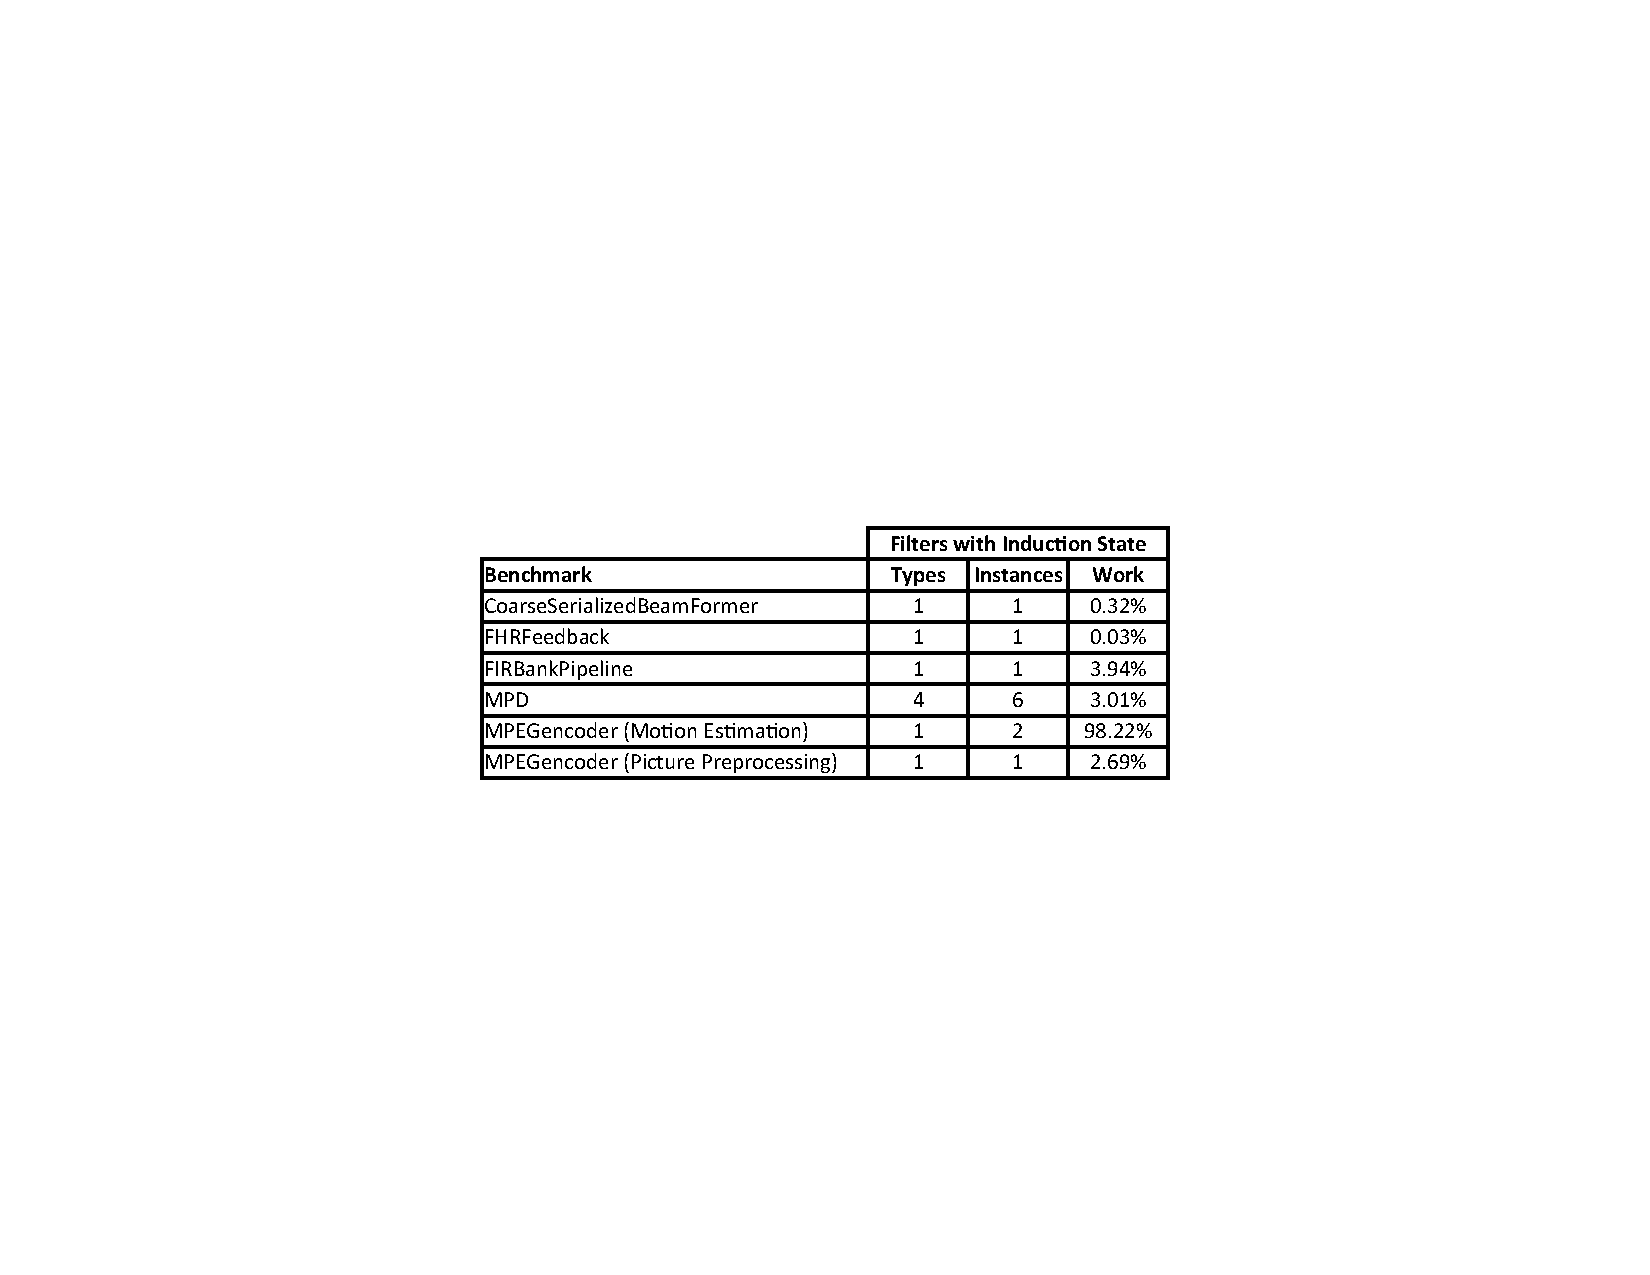
\includegraphics[width=3.3in]{figures/induction-benchmarks.pdf}
\caption{Benchmarks using induction variable state and estimations on work performed in filters with induction state.\protect\label{fig:benchmarks}}
\end{table}


Table~\ref{fig:benchmarks} indicates programs in the StreamIt
benchmark suite that use induction variable filters (not including
source filters) in the manner described above.  The StreamIt compiler
provides static estimations of work performed in filters.  The above
table indicates the percentage of work performed in specifically the induction
variable filters.

The majority of programs do not have substantial work performed in
filters using induction variables; FIRBank and MPD contain only a few
stateful filters whose total work concentration is fairly low.  The
MPEG-2 motion estimation subset is the only exception because its
stream graph is comprised mostly with stateful filters.  However,
eliminating any form of state will have a large impact on runtime
performance even on programs with low work concentration in stateful
filters.  We model the potential speedups of a particular stateful
program in this section.  For the purpose of this analysis, 
assume no communication cost between filters.  Also assume the
compiler exposes no pipeline parallelism.  This assumption forces the
serialization of stateful filters on the stream graph.

Let $N$ be the number of cores we are planning to parallelize over.  Let $\sigma$ be the percentage of work performed in stateful filters that can have its state eliminated, in this case solely filters that use induction variable state.  

If $\sigma = 0$, the entire program is stateless.  The program can be fused to coarsen the granularity, then fissed and mapped to all of the available cores.  Each core would perform $\frac{1}{N}$ of the total work.  Thus with no state, the program can exhibit speedups of up to $N$ times the single-core runtime.

For filters that contain stateful work, $1-\sigma$ of the work in the program is considered stateless, and thus can be fissed and assigned to $N$ individual cores.  The stateful filters cannot be parallelized, and is sequential to all work in the program.  The total serialized work is $\frac{1-\sigma}{N} + \sigma$.  Thus the total speedup is the serial work divided by the new parallelized work.  
\begin{eqnarray*}
\dfrac{1}{\frac{1-\sigma}{N} + \sigma} &=& \dfrac{N}{1 + \sigma(N-1)}
\end{eqnarray*}

We can characterize the amount of speedup between a completely stateless program to an equivalent stateful program with $\sigma$ percentage of stateful work.  This is simply:
\begin{eqnarray*}
\dfrac{N}{\frac{N}{1 + \sigma(N-1)}} &=& 1 + \sigma(N-1)
\end{eqnarray*}

Figure~\ref{fig:theo-speedups} indicates the potential speedups over stateful programs given stateful work percentages and a varying number of cores.  Even benchmarks in the suite that exhibit only 3\% work in stateful filters can exhibit 8x speedups with 256 cores.  Providing a means to remove state from filters that exhibit very small amounts of work relative to the rest of the program can still generate substantial speedups in the near future.

\begin{figure}[t!]
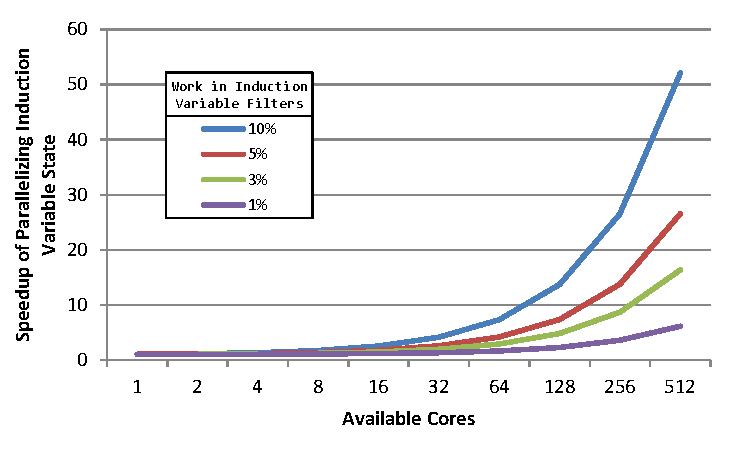
\includegraphics[width=3.3in]{figures/theoretic-speedup.pdf}
\caption{Theoretical speedups of a stateless programs over corresponding
  stateful programs with $\sigma$\% work in filters with explicit
  induction variable state.  \protect\label{fig:theo-speedups}}
\end{figure}
